\documentclass[12pt]{article}

\usepackage{amsmath}
\usepackage{amsfonts}
\usepackage{float}
\usepackage{fancyhdr}
\usepackage{graphicx}
\usepackage[colorlinks=true,linkcolor=blue, citecolor=red]{hyperref}
\usepackage{listings}
\usepackage{url}
\usepackage[top=.75in, left=.5in, right=.5in, bottom=1in]{geometry}
\usepackage{xcolor}
\usepackage[utf8]{vietnam}
\setlength{\headheight}{29.43912pt}
\setlength{\footskip}{29.43912pt}

\graphicspath{{images/}}

\pagestyle{fancy}
\lhead{
Báo cáo Bài tập thực hành 1
}
\rhead{
Trường Đại học Khoa học Tự nhiên - ĐHQG HCM\\
CSC15008 - Xử lý ngôn ngữ tự nhiên ứng dụng
}
\lfoot{\LaTeX\ by \href{https://github.com/trhgquan}{Quan, Tran Hoang}}
% \renewcommand{\footrulewidth}{0.4pt}% default is 0pt


\definecolor{codegreen}{rgb}{0,0.6,0}
\definecolor{codegray}{rgb}{0.5,0.5,0.5}
\definecolor{codepurple}{rgb}{0.58,0,0.82}
\definecolor{backcolour}{rgb}{0.95,0.95,0.92}

\lstdefinestyle{mystyle}{
    backgroundcolor=\color{backcolour},   
    commentstyle=\color{codegreen},
    keywordstyle=\color{magenta},
    stringstyle=\color{codepurple},
    basicstyle=\ttfamily\footnotesize,
    breakatwhitespace=false,         
    breaklines=true,                 
    captionpos=b,                    
    keepspaces=true,                
    showspaces=false,                
    showstringspaces=false,
    showtabs=false,                  
    tabsize=2
}

\lstset{style=mystyle}

\begin{document}

\begin{titlepage}
\newcommand{\HRule}{\rule{\linewidth}{0.5mm}}
\centering

\textsc{\LARGE đại học quốc gia tphcm}\\[1.5cm]
\textsc{\Large trường đại học khoa học tự nhiên}\\[0.5cm]
\textsc{\large khoa công nghệ thông tin}\\[0.5cm]
\textsc{bộ môn công nghệ tri thức}\\[0.5cm]

\HRule \\[0.4cm]
{ 
\huge{\bfseries{Báo cáo Bài tập thực hành 01}}\\[0.5cm]
\large{\bfseries{Đề tài: Tìm hiểu công cụ KenLM}}
}\\[0.4cm]
\HRule \\[0.5cm]

\textbf{\large Môn học: CSC15008 - Xử lý ngôn ngữ tự nhiên ứng dụng}\\[0.5cm]

\begin{minipage}{0.4\textwidth}
\begin{flushleft} \large
\emph{Sinh viên thực hiện:}\\
Trần Hoàng Quân \textsc{(19120338)}
% Nguyễn Văn A \textsc{(19120000)}
\end{flushleft}
\end{minipage}
~
\begin{minipage}{0.4\textwidth}
\begin{flushright} \large
\emph{Giáo viên hướng dẫn:} \\
% Dr. James \textsc{Smith}
Thầy Nguyễn Hồng Bửu Long
\end{flushright}
\end{minipage}\\[2cm]

{\large \today}\\[2cm]


\includegraphics{hcmus-logo.png}\\[1cm] 

\vfill
\end{titlepage}
	
\tableofcontents
\pagebreak

\section{Giới thiệu công cụ KenLM}
KenLM Language Model Toolkit là công cụ xây dựng mô hình ngôn ngữ (language models) phát triển bởi nhà nghiên cứu Kenneth Heafield đến từ Đại học Edinburgh, Scotland. Công cụ có thể tính toán, lọc và truy vấn trên các mô hình ngôn ngữ. Một số ưu điểm của bộ công cụ có thể kể đến:
\begin{itemize}
\item Truy vấn nhanh và sử dụng ít bộ nhớ.\cite{heafield-2011-kenlm}
\item Tính toán ước lượng rất nhanh, dễ mở rộng.\cite{heafield-etal-2013-scalable}
\end{itemize}
Thông tin của bộ công cụ có thể đọc thêm tại đây:
\begin{itemize}
\item Trang chủ của công cụ: \href{https://kheafield.com/code/kenlm}{https://kheafield.com/code/kenlm}.
\item GitHub repository: \href{https://github.com/kpu/kenlm}{https://github.com/kpu/kenlm}
\end{itemize}
\subsection{Cài đặt \& biên dịch}
Báo cáo được thực hiện với môi trường Ubuntu 21.10.
\begin{enumerate}
\item Trên môi trường Ubuntu, clone GitHub repository của project về:
\begin{lstlisting}[language=sh]
git clone git@github.com:kpu/kenlm.git
\end{lstlisting}

\item KenLM được viết bằng C++, sử dụng một số thư viện hỗ trợ như Boost và biên dịch bằng cmake. Vì vậy, ta cần cài đặt các thư viện hỗ trợ. Tiến hành cài như sau:
\begin{lstlisting}[language=sh]
sudo apt install build-essential cmake libboost-system-dev libboost-thread-dev libboost-program-options-dev libboost-test-dev libeigen3-dev zlib1g-dev libbz2-dev liblzma-dev
\end{lstlisting}

\item Build bản executable:
\begin{lstlisting}[language=sh]
cd kenlm
mkdir -p build && cd build
cmake ..
make -j 4
\end{lstlisting}
\item File thực thi sau khi build sẽ nằm trong thư mục \texttt{kenlm/build}
\end{enumerate}
\subsection{Hướng dẫn sử dụng}

\subsubsection{Huấn luyện \& sử dụng model}
KenLM sẽ tạo một $n$-gram model dựa trên tập dữ liệu đầu vào \texttt{text}, sau đó lưu model vào file \texttt{text.arpa}. Sử dụng câu lệnh sau để tiến hành train:
\begin{lstlisting}[language=sh]
./bin/lmplz -o n <text >text.arpa
\end{lstlisting}
Ví dụ, ta cần tạo một 3-gram model từ tập tin \texttt{input.in}, lưu ra tập tin \texttt{build/model.arpa}. Khi đó câu lệnh trở thành:
\begin{lstlisting}[language=sh]
./bin/lmplz -o 3 <text.in >model.arpa
\end{lstlisting}
Để sử dụng: ta chỉ cần chạy câu lệnh sau để truy vấn điểm và perplexity của một câu (VD: \texttt{this is a sample sentence .}):
\begin{lstlisting}[language=sh]
echo "this is a sample sentence ." | ./bin/query model.arpa
\end{lstlisting}

\subsubsection{Score}
Điểm (score) của một câu $W: w_1w_2..w_N$ gồm $N$ từ được tính theo công thức:
$$
P(W) = P(w_1)P(w_2|w_1)P(w_3|w_1w_2)..P(w_N|w_1w_2..w_{N - 1})\footnote{$P(w_i|w_1w_2..w_{i - 1})$ là xác suất từ $w_i$ xuất hiện nếu các từ trước đó lần lượt là $w_1w_2..w_{i - 1}; P(w_i)$ là xác suất từ $w_i$ xuất hiện.} \approx \prod_{i = 1}^N P(w_i | w_1w_2..w_{i - 1})
$$
Lấy $\log$ hai vế:
$$
\log(P(W)) \approx \sum_{i = 1}^{N} \log(P(w_i | w_1w_2..w_{i - 1}))
$$
Mặc định khi sử dụng lệnh \texttt{query} KenLM sẽ đưa ra điểm (đã lấy $\log$) của toàn câu.

\subsubsection{Perplexity}
Perplexity của một câu $W: w_1w_2..w_N$ gồm $N$ từ được tính theo công thức:
$$
\displaystyle
\text{perplexity}(W) = \sqrt[N]{\prod_{i = 1}^{N} \frac{1}{P(w_i | w_1w_2..w_{i - 1})}} = \sqrt[N]{\frac{1}{10^{\log(P(W))}}}
$$
Mặc định khi sử dụng lệnh \texttt{query} KenLM sẽ đưa ra perplexity của toàn câu, cùng với perplexity khi đã loại các OOV\footnote{out of vocabulary words - từ ngoài từ điển}.


\subsubsection{Cấu trúc file ARPA}
ARPA là định dạng file lưu các mô hình ngôn ngữ. Người dùng có dễ dàng mở bằng các công cụ chỉnh sửa file text để đọc và tính toán. Mở đầu của dữ liệu mô hình ngôn ngữ lưu trong file ARPA là chuỗi 6 byte:
\begin{lstlisting}
\\data\\
\end{lstlisting}
Các dòng tiếp theo là số lượng của mỗi loại $n$-gram. Ví dụ:
\begin{lstlisting}
ngram 1=500
ngram 2=1250
ngram 3=2500
\end{lstlisting}
Các dòng theo sau, mỗi dòng lần lượt là xác suất, từ và backoff weight của từng từ. Ví dụ cho model 3-gram:
\begin{lstlisting}
\1-grams:
log10_prob(word1) word1 log10_backoff(word1)
log10_prob(word2) word2 log10_backoff(word2)
...
\2-grams:
log10_prob(word1|word1) word1 word1 log10_backoff(word1,word1)
log10_prob(word1|word2) word2 word1 log10_backoff(word2,word1)
log10_prob(word2|word1) word1 word2 log10_backoff(word1,word2)
...
\3-grams:
log10_prob(word3|word1,word2) word1 word2 word3
...
\end{lstlisting}
Nội dung file kết thúc bởi chuỗi
\begin{lstlisting}
\end\
\end{lstlisting}
Cấu trúc file ARPA được tham khảo từ tài liệu của UCBerkeley \cite{arpa-definition}.
Một số lưu ý: 
\begin{itemize}
\item Xác suất \texttt{log10\_prob} được tính theo $\log_{10}$ \footnote{log thập phân, thường viết gọn là $\log$}. Ví dụ, nếu xác suất $P(w_i) = 0.00028$ thì $\texttt{log10\_prob}(w_i)= \log(0.00028) = -3.55284196866$. Do đó, nếu muốn tính xác suất thực thì phải lấy $10^{\texttt{log10\_prob}}$.
\item Backoff weight sẽ được giải thích và tính toán kỹ hơn với ví dụ ở phần \ref{danhgia-noov}. Cơ bản là nếu xác suất $n$-gram bằng 0 thì ta sẽ quay lui về tính xác suất $(n - 1)$-gram, sau đó cộng thêm giá trị backoff weight của $(n - 1)$-gram. Nếu $(n - 1)$-gram tiếp tục bằng 0 thì lại lùi về $(n - 2)$-gram.
\end{itemize}

\section{Thực hành Huấn luyện và đánh giá model với KenLM}
Data mẫu được trích từ bản dịch tiếng Anh tác phẩm Con Đầm Pích của nhà văn Nga Aleksandr Sergeyevich Pushkin \cite{queen-of-spades}. Phần data dùng để huấn luyện đã qua tiền xử lý gồm các bước như sau:
\begin{itemize}
\item Bỏ qua phần thông tin đính kèm của Project Gutenberg.
\item Loại bỏ các dấu xuống dòng thừa. Data nguyên bản ngắt dòng trong đoạn văn để căn chỉnh độ rộng của nội dung.
\item Chuyển tất cả các ký tự về chữ thường.
\item Thêm dấu cách để phân biệt punctuations (dấu câu) và các từ.
\end{itemize}
Data (trước và sau preprocess) cùng với file model ARPA có thể download ở \href{https://studenthcmusedu-my.sharepoint.com/:f:/g/personal/19120338_student_hcmus_edu_vn/EqFiWm6iywdKms6WFubsNOYBOzqfFttfH8P81jBT8gcZIw?e=truaMM}{link này}\label{download-model}.

\subsection{Huấn luyện}
Chúng ta tiến hành huấn luyện model 3-gram ($n = 3$)
\begin{lstlisting}[language=sh]
./bin/lmplz -o 3 <../../CS158/queenofspades.txt >model.arpa
\end{lstlisting}
kết quả huấn luyện rất nhanh - chưa đến 1 giây:
\begin{figure}[H]
\centering {
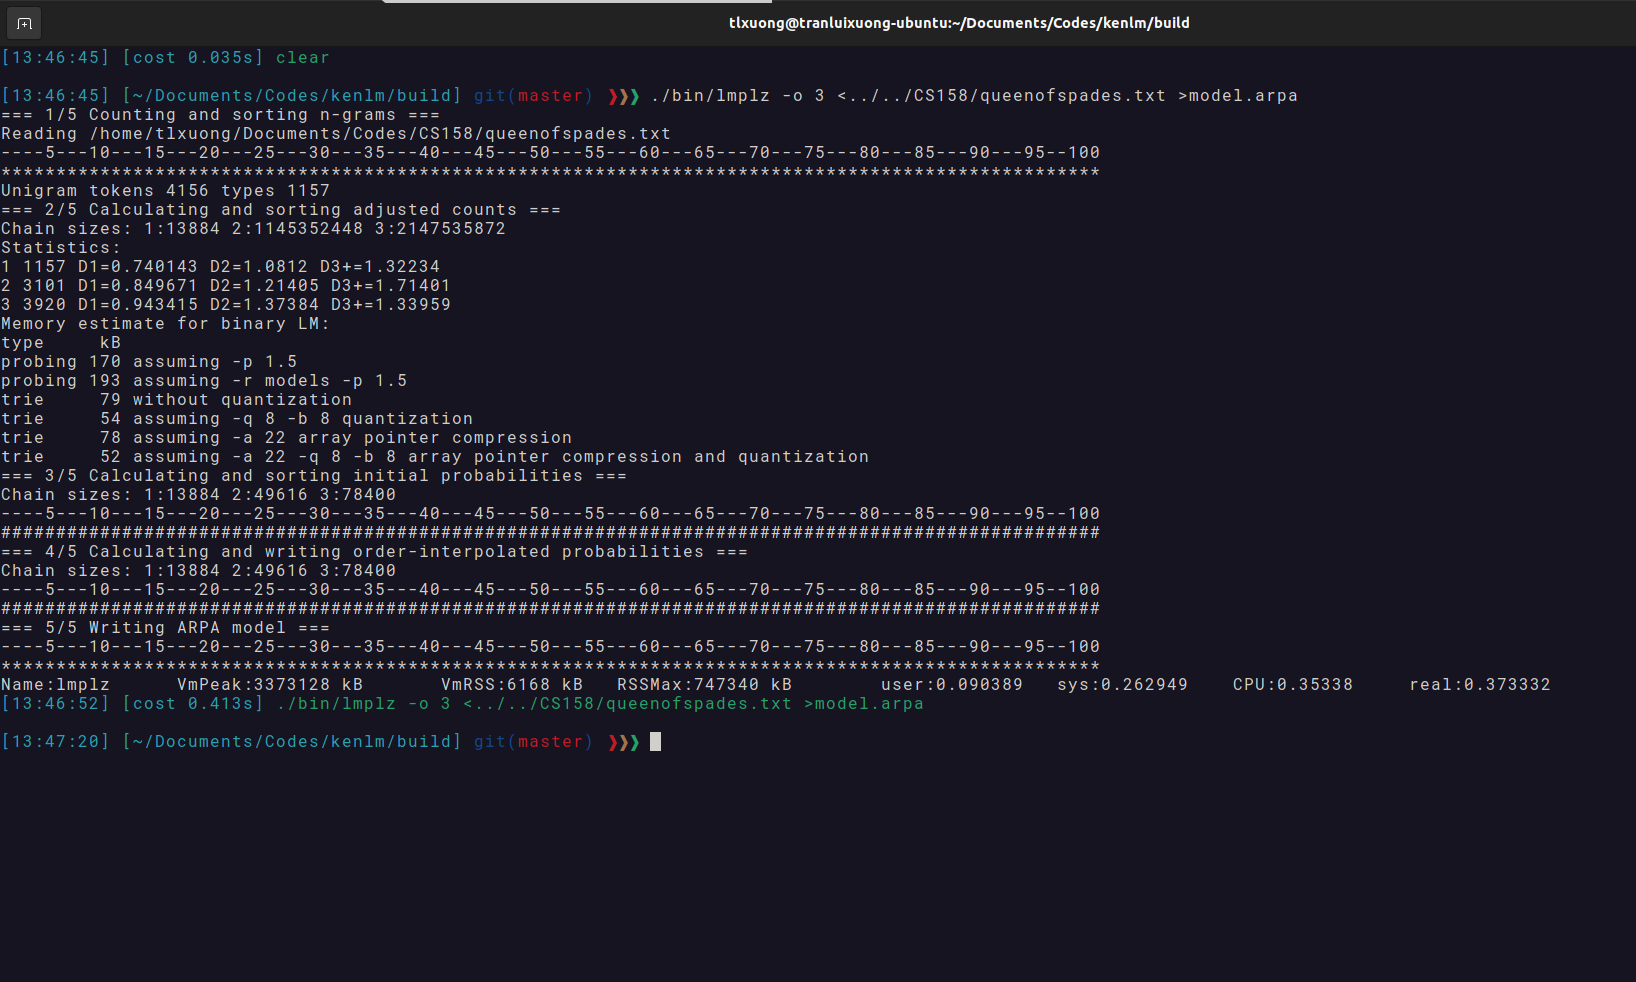
\includegraphics[scale=.55]{ket-qua-huan-luyen.PNG}
\caption{Kết quả huấn luyện}
}
\end{figure}
\noindent Các thông số huấn luyện lần lượt là số lượng unigram, bigram và trigram trong model:
\begin{table}[H]
\centering
\begin{tabular}{|c|c|c|}
    \hline
    Unigram & Bigram & Trigram \\
    \hline
    1157 & 3101 & 3920 \\
    \hline
\end{tabular}
\caption{Các thông số sau khi huấn luyện}
\end{table}
\subsection{Đánh giá model}
\subsubsection{Câu trong văn bản}\label{danhgia-noov}
Ta thử với câu \texttt{my grandmother never gambles .}, câu này xuất hiện trong cuộc đối thoại giữa nhân vật Herman và Tomsky. Tiến hành truy vấn như sau:
\begin{lstlisting}[language=sh]
echo "my grandmother never gambles ." | ./bin/query model.arpa
\end{lstlisting}
\begin{figure}[H]
\centering {
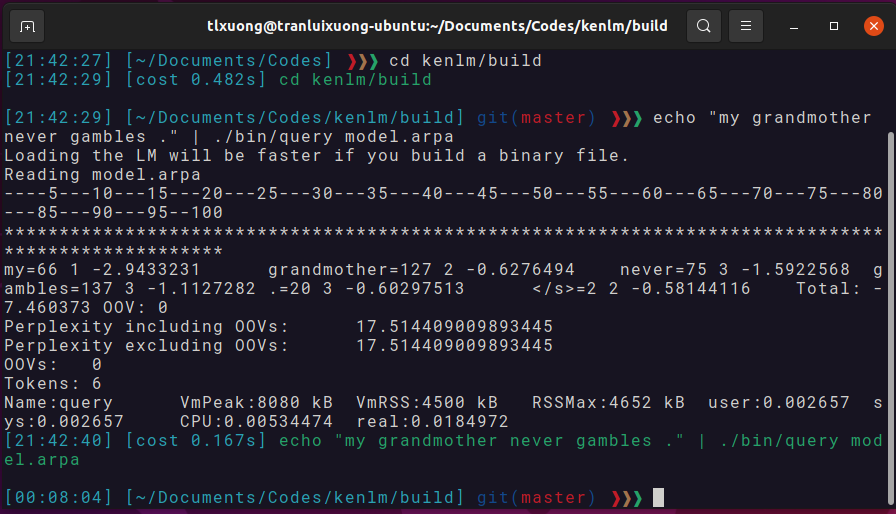
\includegraphics{ba-toi-khong-danh-bac.PNG}
\caption{Kết quả truy vấn câu \texttt{my grandmother never gambles.}}
}
\end{figure}
\noindent Kết quả được tổng hợp thành bảng sau:
\begin{table}[H]
\centering
\begin{tabular}{|c|c|c|}
    \hline
    Từ & $n$-gram & Xác suất \\
    \hline
    my & 1 & -2.9433231\\
    grandmother & 2 & -0.6276494\\
    never & 3 & -1.5922568\\
    gambles & 3 & -1.1127282\\
    . & 3 & -0.60297513\\
    \texttt{</s>} (dấu kết câu) & 2 & -0.58144116\\
    \hline
\end{tabular}
\caption{Kết quả đánh giá câu \texttt{my grandmother never gambles.}}
\label{table:2}
\end{table}
\begin{table}[h!]
\centering
\begin{tabular}{|c|c|}
    \hline
    Nội dung & Kết quả \\
    \hline
    Tổng điểm (total score) & -7.460373 \\
    Perplexity & 17.514409009893445\\
    Perplexity, đã loại OOVs & 17.514409009893445\\
    OOVs & 0 \\
    \hline
\end{tabular}
\caption{Kết quả đánh giá câu \texttt{my grandmother never gambles.}(tt.)}
\end{table}
\noindent Chú ý: xem lại phần \ref{download-model} để tra cứu file ARPA. Cách tính bảng \ref{table:2} như sau:
\begin{itemize}

\item Từ \texttt{my}: xét cụm \texttt{<s> my}, cụm này không có trong từ điển. Khi đó 
$$P(\texttt{my | <s>}) = P(\texttt{my}) + B(\texttt{<s>})\footnote{$B(w_i | w_1w_2..w_{i - 1})$ là giá trị backoff của câu $w_1w_2..w_i$; $B(w_i)$ là giá trị backoff của từ $w_i$} = -2.392768 - 0.55055535 \approx -2.9433231$$
Vì chúng ta backoff từ 2-gram về 1-gram, nên ở đây giá trị $n = 1$.

\item Từ \texttt{mother}: xét cụm \texttt{<s> my grandmother}, cụm này không có trong từ điển. Bù lại, ta đã có $P(\texttt{grandmother | my}) = -0.6276494; P(\texttt{my | <s>})$ đã tính bên trên, nên cụm \texttt{my <s>} xem như đã tồn tại và có giá trị backoff bằng 0. Do đó,
$$P(\texttt{grandmother | <s> my}) = -0.6276494 + 0 = -0.6276494$$
Ta backoff từ 3-gram về 2-gram, nên giá trị $n = 2$.

\item Từ \texttt{never}: xét cụm \texttt{my grandmother never} đã tồn tại trong model và có xác suất bằng -1.5922568. Vì vậy
$$P(\texttt{never | my grandmother}) = -1.5922568$$
Ở đây không backoff nên $n = 3$. Ta tính toán tương tự với các từ \texttt{gambles} và dấu \texttt{.}

\item Dấu kết câu \texttt{<s>}: cụm \texttt{gambles . </s>} không có trong từ điển, nên
$$
P(\texttt{</s> | gambles .)} = P(\texttt{</s> | .)} + B(\texttt{. | gambles})
$$
$$
= -0.556144 -0.025297174 \approx -0.58144116
$$
vì backoff từ 3-gram về 2-gram nên $n = 2$.
\end{itemize}
Các giá trị như điểm (total score), perplexity của câu: cách tính đã nêu bên trên nên không được đề cập ở đây.
\subsubsection{Câu ngoài văn bản}
Ta chọn câu \texttt{my grandfather never gambles .} Câu lệnh truy vấn như sau:
\begin{lstlisting}[language=sh]
echo "my grandfather never gambles ." | ./bin/query model.arpa
\end{lstlisting}
\begin{figure}[H]
\centering {
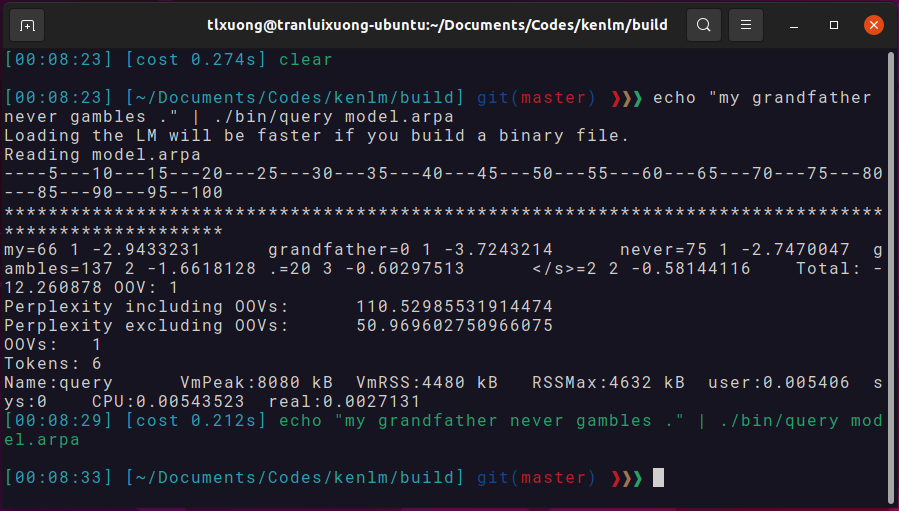
\includegraphics{ong-toi-khong-danh-bac.PNG}
\caption{Kết quả truy vấn câu \texttt{my grandfather never gambles.}}
}
\end{figure}
\noindent Kết quả được tổng hợp thành bảng sau:
\begin{table}[H]
\centering
\begin{tabular}{|c|c|c|}
    \hline
    Từ & $n$-gram & Xác suất \\
    \hline
    my & 1 & -2.9433231\\
    grandfather & 1 & -3.7243214\\
    never & 1 & -2.7470047\\
    gambles & 2 & -1.6618128\\
    . & 3 & -0.60297513\\
    \texttt{</s>} (dấu kết câu) & 2 & -0.58144116\\
    \hline
\end{tabular}
\caption{Kết quả đánh giá câu \texttt{my grandfather never gambles.}}
\label{table:4}
\end{table}
\begin{table}[h!]
\centering
\begin{tabular}{|c|c|}
    \hline
    Nội dung & Kết quả \\
    \hline
    Tổng điểm (total score) & -12.260878 \\
    Perplexity & 110.52985531914474\\
    Perplexity, đã loại OOVs & 50.969602750966075\\
    OOVs & 1 \\
    \hline
\end{tabular}
\caption{Kết quả đánh giá câu \texttt{my grandfather never gambles.}(tt.)}
\end{table}
\noindent Kết quả tính toán bảng \ref{table:4} có sự khác biệt:
\begin{itemize}
\item Từ \texttt{grandfather} hoàn toàn không có trong từ điển, nên 
$$
P(\texttt{grandfather | my}) = P(\texttt{<unk>}) + B(\texttt{my}) = -3.5495179 - 0.17480342 \approx -3.7243214
$$
\item Các từ khác tính toán tương tự mục \ref{danhgia-noov}.
\end{itemize}
KenLM sử dụng từ \texttt{<unk>} để đánh dấu một từ chưa từng xuất hiện trong từ điển, từ này cũng có điểm thấp hơn các từ khác. Điều này dẫn tới total score của câu thấp hơn, perplexity cao hơn câu \texttt{my grandmother never gambles .} bên trên.

\section{Mở rộng: Sử dụng package kenlm trên Python3}\label{python-kenlm}
\subsection{Cài đặt \& sử dụng}
Ta có thể sử dụng package \texttt{kenlm} trong Python. Tiến hành cài đặt package thông qua \texttt{pip}:
\begin{lstlisting}[language=sh]
pip install https://github.com/kpu/kenlm/archive/master.zip
\end{lstlisting}
Sau khi cài đặt, ta có thể load model lên để sử dụng:
\begin{lstlisting}[language=python]
import kenlm

# Nho chep file build/model.arpa vao thu muc cung cap voi script Python!
model = kenlm.Model('model.arpa')

# In model score cho mot cau.
print(model.score('this is a sample sentence .', bos = True, eos = True))
\end{lstlisting}

\subsection{Tính perplexity}
Nếu sử dụng module \texttt{kenlm} trong Python, ta có một bộ các giá trị $p_i$ đã được tính toán sẵn và có thể truy xuất thông qua method \texttt{kenlm.Model.full\_scores(str)}. Quá trình tính được cài đặt như sau:
\begin{lstlisting}[language=python]
import kenlm
import math

model = kenlm.Model('model.arpa')
s = 'this is a sample sentence .'
score_list = [score for score, _, _ in model.full_scores(s)]

# Tinh tich cac prod (mu 10 vi kenlm mac dinh lay log10(prod)
inverse_product = 1

for score in score_list:
    inverse_product *= math.pow(10.0, score)

# Tinh inverse cua prod
inverse_product = 1 / inverse_product

# Tinh perplexity = nroot(inverse_prod) = inverse_prod ^ (1/n)
perplexity = math.pow(inverse_product, 1.0 / len(score_list))

print('Perplexity of sentence {0} is: {1}', s, perplexity)
\end{lstlisting}
Ngoài ra, ta có thể sử dụng method \texttt{kenlm.Model.perplexity(str)} đã được cài đặt sẵn\footnote{Chú ý là cách này không tính tag bắt đầu (\texttt{<s>}) / kết thúc câu (\texttt{</s>}) như là một từ. Tham khảo đoạn code tính \href{https://github.com/kpu/kenlm/blob/217e219a34f8ac5d096b2fff3dede82b5a182a88/python/kenlm.pyx\#L209-L215}{tại đây}}:
\begin{lstlisting}[language=python]
import kenlm

model = kenlm.Model('model.arpa')
s = 'this is a sample sentence .'
perplexity = model.perplexity(s)

print('Perplexity of sentence {0} is: {1}', s, perplexity)
\end{lstlisting}

\begin{figure}[h]
    \centering
    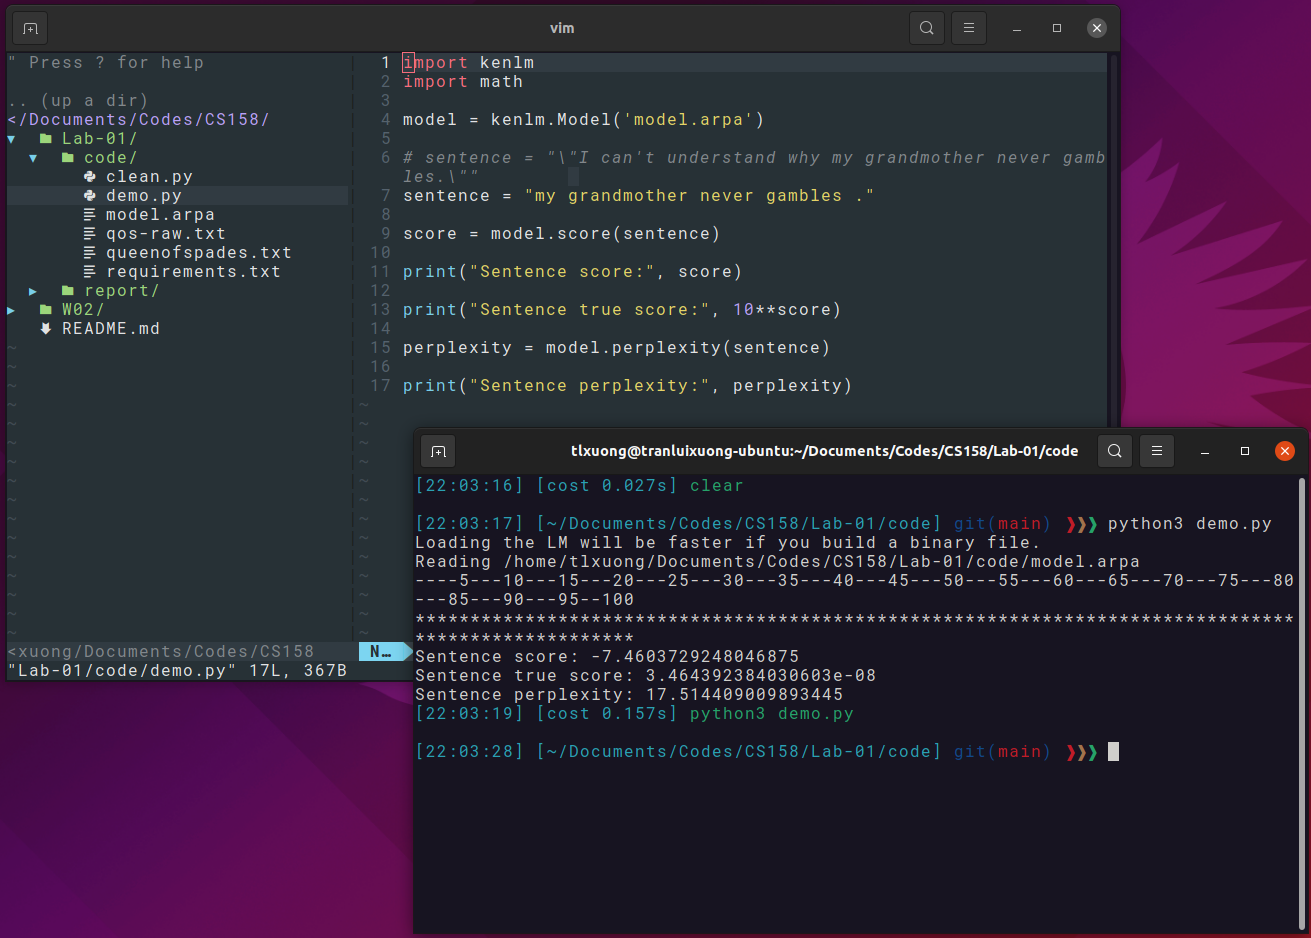
\includegraphics[scale=.70]{python-demo.PNG}
    \caption{Demo package kenlm trên Python}
\end{figure}

\section{Kết luận}
\begin{itemize}
\item KenLM huấn luyện và truy vấn rất nhanh trên mô hình.
\item Các câu không hợp lệ dễ phát hiện (total score thấp, perplexity cao).
\end{itemize}
\noindent Nhìn chung, KenLM là một công cụ có hiệu năng cao, độ chính xác đáng tin cậy, rất đáng sử dụng.

\cleardoublepage
\phantomsection
\addcontentsline{toc}{section}{Tài liệu}
\bibliographystyle{plain}
\bibliography{sample}

\end{document}